\documentclass[a4paper,10pt]{book}
\usepackage{doxygen_custom}
\usepackage{enumitem}
\setlist[1]{itemsep=-5pt,topsep=0pt}

\usepackage{titlesec}

%\titleformat{command}[shape]{format}{label}{sep}{before}[after]
%\titleformat{\section}      [runin]{\normalfont\LARGE\bfseries}{\thesection}{}{}
%\titleformat{\subsection}   [runin]{\normalfont\Large\bfseries}{\thesubsection}{}{}
\titleformat{\subsubsection}[runin]{\normalfont\bfseries}{\thesubsubsection}{1em}{}[.]


%\newcommand{\chaptermark}{}
\usepackage{a4wide}
\usepackage{makeidx}
\usepackage{graphicx}
\usepackage{multicol}
\usepackage{float}
\usepackage{listings}
\usepackage{color}
\usepackage{textcomp}
\usepackage{alltt}
\usepackage{times}
\usepackage{ifpdf}


\ifpdf
\usepackage[pdftex,
            pagebackref=true,
            colorlinks=true,
            linkcolor=blue,
            unicode
           ]{hyperref}
\else
\usepackage[ps2pdf,
            pagebackref=true,
            colorlinks=true,
            linkcolor=blue,
            unicode
           ]{hyperref}
\usepackage{pspicture}
\fi
\usepackage[utf8]{inputenc}



% Replace doxygen fancy header (set in doxygen package) with our own
\lhead[\fancyplain{}{\bfseries\thepage}]{DMP Tutorial}%
\rhead[\fancyplain{}{\bfseries\thepage}]{\footnotesize Freek Stulp}%
\rfoot[\fancyplain{}{\bfseries\thepage}]{\footnotesize ENSTA-ParisTech}%

\lstset{language=C++,inputencoding=utf8,basicstyle=\footnotesize,breaklines=true,breakatwhitespace=true,tabsize=8,numbers=left}

\setcounter{secnumdepth}{-1} 

% My preferred font
\sffamily 
\renewcommand{\rmdefault}{phv} % Arial
\renewcommand{\sfdefault}{phv} % Arial




\graphicspath{{../images/}}

\author{Freek Stulp}
\title{Dynamical Movement Primitives Tutorial}

\begin{document}

\maketitle

This document was generated by doxygen, so the formatting is not always optimized for pdflatex.

\setcounter{tocdepth}{2}
\tableofcontents

\newpage



%This library contains several modules for training dynamical movement primitives (D\+M\+Ps), and optimizing their parameters through black-\/box optimization. Each module has its own dedicated page.

\begin{DoxyItemize}
\item \hyperlink{page_dyn_sys}{Dynamical Systems Module} This module provides implementations of several basic dynamical systems. D\+M\+Ps are combinations of such systems. This module is completely independent of all other modules.\end{DoxyItemize}
\begin{DoxyItemize}
\item \hyperlink{page_func_approx}{Function Approximation Module} This module provides implementations (but mostly wrappers around external libraries) of several function approximators. D\+M\+Ps use function approximators to learn and reproduce arbitrary smooth movements. This module is completely independent of all other modules.\end{DoxyItemize}
\begin{DoxyItemize}
\item \hyperlink{page_dmp}{Dynamical Movement Primitives Module} This module provides an implementation of several types of D\+M\+Ps. It depends on both the Dynamical\+Systems and Function\+Approximators modules, but no other.\end{DoxyItemize}
\begin{DoxyItemize}
\item \hyperlink{page_bbo}{Black Box Optimization} This module provides implementations of several stochastic optimization algorithms for the optimization of black-\/box cost functions. This module is completely independent of all other modules.\end{DoxyItemize}
\begin{DoxyItemize}
\item \hyperlink{page_dmp_bbo}{Black Box Optimization of Dynamical Movement Primitives} This module applies black-\/box optimization to the parameters of a D\+M\+P. It depends on all the other modules.\end{DoxyItemize}
Each of the pages linked to above contains two sections\+:

\begin{DoxyItemize}
\item A tutorial that treats the concepts that are implemented \item A description of how these concepts have been implemented, and why it has been done so in this fashion.\end{DoxyItemize}
If you want a deeper understanding of the entire library, I recommend you to go through the pages in the order above. If you want to start coding immediately, I suggest to look at the \hyperlink{group__Demos}{Demos} to see how the functionality of the library may be used. The demos for each module are found in cpp/\+M\+O\+D\+U\+L\+E\+N\+A\+M\+E/demos.

Some general considerations on the design of the library are here \hyperlink{page_design}{Design Rationale} 
%
%\newpage

\chapter{Dynamical Systems}
\hypertarget{page_dyn_sys_sec_dyn_sys_intro}{}\subsection{Introduction}\label{page_dyn_sys_sec_dyn_sys_intro}
Let a {\itshape state} be a vector of real numbers. A dynamical system consists of such a state and a rule that describes how this state will change over time; it describes what future state follows from the current state. A typical example is radioactive decay, where the state $x$ is the number of atoms, and the rate of decay is $\frac{dx}{dt}$ proportional to $x$\+: $ \frac{dx}{dt} = -\alpha x$. Here, $\alpha$ is the `decay constant' and $\dot{x}$ is a shorthand for $\frac{dx}{dt}$. Such an evolution rule describes an implicit relation between the current state $ x(t) $ and the state a short time in the future $x(t+dt)$.

If we know the initial state of a dynamical system, e.\+g. $x_0\equiv x(0)=4$, we may compute the evolution of the state over time through {\itshape numerical} {\itshape integration}. This means we take the initial state $ x_0$, and iteratively compute subsequent states $x(t+dt)$ by computing the rate of change $\dot{x}$, and integrating this over the small time interval $dt$. A pseudo-\/code example is shown below for $x_0\equiv x(0)=4$, $dt=0.01s$ and $\alpha=6$.


\begin{DoxyCode}
alpha=6; \textcolor{comment}{// Decay constant}
dt=0.01; \textcolor{comment}{// Duration of one integration step}
x=4.0;   \textcolor{comment}{// Initial state}
t=0.0;   \textcolor{comment}{// Initial time}
\textcolor{keywordflow}{while} (t<1.5) \{
  dx = -alpha*x;  \textcolor{comment}{// Dynamical system rule}
  x = x + dx*dt;  \textcolor{comment}{// Project x into the future for a small time step dt (Euler integration)}
  t = t + dt;     \textcolor{comment}{// The future is now!}
\}
\end{DoxyCode}


This procedure is called ``integrating the system'', and leads the trajectory plotted below (shown for both $\alpha=6$ and $\alpha=3$.


\begin{DoxyImage}
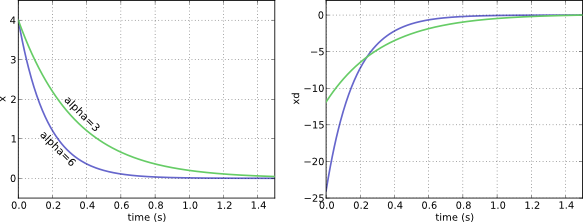
\includegraphics[height=4cm]{exponential_decay-svg}
\caption{Evolution of the exponential dynamical system.}
\end{DoxyImage}


The evolution of many dynamical systems can also be determined analytically, by explicitly solving the differential equation. For instance, $N(t) = x_0e^{-\alpha t}$ is the solution to $\dot{x} = -\alpha x$. Why? Let's plug $x(t) = x_0e^{-\alpha t}$ into $\frac{dx}{dt} = -\alpha x$, which leads to $\frac{d}{dt}(x_0e^{-\alpha t}) = -\alpha (x_0e^{-\alpha t})$. Then derive the left side of the equations, which yields $-\alpha(x_0e^{-\alpha t}) = -\alpha (x_0e^{-\alpha t})$. Q\+E\+D. Note that the solution works for arbitrary $x_0$. It should, because the solution should not depend on the initial state.\hypertarget{page_dyn_sys_dynsys_implementation1}{}\subsubsection{Implementation}\label{page_dyn_sys_dynsys_implementation1}
{\itshape  In the object-\/oriented implementation of this module, all dynamical systems inherit from the abstract Dynamical\+System class. The analytical solution of a dynamical system is computed with Dynamical\+System\+::analytical\+Solution, which takes the times {\ttfamily ts} at which the solution should be computed, and returns the evolution of the system as {\ttfamily xs} and {\ttfamily xds}.}

{\itshape A system's differential equation is implement in the function Dynamical\+System\+::differential\+Equation, which takes the current state {\ttfamily x}, and computes the rates of change {\ttfamily xd}. The functions Dynamical\+System\+::integrate\+Start() and Dynamical\+System\+::integrate\+Step() are then used to numerically integrate the system as follows (using the example plotted above)\+:}

{\itshape 
\begin{DoxyCode}
\textcolor{comment}{// Make exponential system that decays from 4 to 0 with decay constant 6, and tau=1.0}
\textcolor{keywordtype}{double} alpha = 6.0;                \textcolor{comment}{// Decay constant}
\textcolor{keywordtype}{double} tau = 1.0;                  \textcolor{comment}{// Time constant }
VectorXd x\_init(1); x\_init << 4.0; \textcolor{comment}{// Initial state (a 1D vector with the value 4.0 inside using Eigen
       comma initializer)}
VectorXd x\_attr(1); x\_attr << 0.0; \textcolor{comment}{// Attractor state}
DynamicalSystem* dyn\_sys = \textcolor{keyword}{new} ExponentialSystem(tau, x\_init, x\_attr, alpha);

Eigen::VectorXd x, xd;
dyn\_sys->integrateStart(x,xd); \textcolor{comment}{// Start the integration}
\textcolor{keywordtype}{double} dt = 0.01;
\textcolor{keywordflow}{for} (\textcolor{keywordtype}{double} t=0.0; t<1.5; t+=dt)
\{
  dyn\_sys->integrateStep(dt,x,x,xd);          \textcolor{comment}{// Takes current state x, integrates system, and writes next
       state in x, xd}
  cout << t << \textcolor{stringliteral}{" "} << x << \textcolor{stringliteral}{" "} << xd << endl; \textcolor{comment}{// Output current time, state and rate of change}
\}
\textcolor{keyword}{delete} dyn\_sys;
\end{DoxyCode}
}

{\itshape {\itshape Remark}. Both analytical\+Solution and differential\+Equation functions above are const, i.\+e. they do not change the Dynamical\+System itself.}

{\itshape {\itshape Remark}. Dynamical\+System\+::integrate\+Step uses either Euler integration, or 4-\/th order Runge-\/\+Kutta. The latter is more accurate, but requires 4 calls of Dynamical\+System\+::differential\+Equation() instead of 1). Which one is used can be set with Dynamical\+System\+::set\+\_\+integration\+\_\+method(). To numerically integrate a dynamical system, one must carefully choose the integration time dt. Choosing it too low leads to inaccurate integration, and the numerical integration will diverge from the 'true' solution acquired through analytical solution. See \href{http://en.wikipedia.org/wiki/Euler%27s_method}{\tt http\+://en.\+wikipedia.\+org/wiki/\+Euler\%27s\+\_\+method} for examples. Choosing dt depends entirely on the time-\/scale (seconds vs. years) and parameters of the dynamical system (time constant, decay parameters).}

{\itshape }\hypertarget{page_dyn_sys_dynsys_implementation1_plotting}{}\subsubsection{Plotting}\label{page_dyn_sys_dynsys_implementation1_plotting}
{\itshape  If you save the output of a dynamical in a file with format (where D is the dimensionality of the system, and T is the number of time steps) \begin{DoxyVerb}x^0_0 x^1_0 .. x^D_0   xd^0_0 xd^1_0 .. xd^D_0   t_0   
x^0_1 x^1_1 .. x^D_1   xd^0_1 xd^1_1 .. xd^D_1   t_1   
   :     :       :         :      :       :       :    
x^0_T x^1_T .. x^D_T   xd^0_T xd^1_T .. xd^D_T   t_T   
\end{DoxyVerb}
 you can plot this output with 
\begin{DoxyCode}
python dynamicalsystems/plotting/plotDynamicalSystem.py file.txt
\end{DoxyCode}
}

{\itshape }\hypertarget{page_dyn_sys_dynsys_implementation1_demo}{}\subsubsection{Demos}\label{page_dyn_sys_dynsys_implementation1_demo}
{\itshape  A demonstration of how to initialize and integrate an Exponential\+System is in \hyperlink{demoExponentialSystem_8cpp}{demo\+Exponential\+System.\+cpp}}

{\itshape A more complete demonstration including all implemented dynamical systems is in \hyperlink{demoDynamicalSystems_8cpp}{demo\+Dynamical\+Systems.\+cpp}. If you call the resulting executable with a directory argument, e.\+g. 
\begin{DoxyCode}
./demoDynamicalSystems /tmp/demoDynamicalSystems
\end{DoxyCode}
 it will save results to file, which you can plot with for instance\+: 
\begin{DoxyCode}
python plotDynamicalSystem.py /tmp/demoDynamicalSystems/ExponentialSystem/results\_rungekutta.txt
python plotDynamicalSystem.py /tmp/demoDynamicalSystems/ExponentialSystem/results\_euler.txt
\end{DoxyCode}
 Different test can be performed with the dynamical system. The test can be chosen by passing further argument, e.\+g. 
\begin{DoxyCode}
./demoDynamicalSystems /tmp/demoDynamicalSystems rungekutta euler
\end{DoxyCode}
 will integrate the dynamical systems with both the Runge-\/\+Kutta and simple Euler method. The available tests are\+: \begin{DoxyItemize}
\item \char`\"{}rungekutta\char`\"{} -\/ Use 4th-\/order Runge-\/\+Kutta integration (more accurate, but more calls of Dynamical\+System\+::differential\+Equation) \item \char`\"{}euler\char`\"{} -\/ Use simple Euler integration (less accurate, but faster) \item \char`\"{}analytical\char`\"{} -\/ Use the analytical solution instead of numerical integration \item \char`\"{}tau\char`\"{} -\/ Change tau before doing numerical integration \item \char`\"{}attractor\char`\"{} -\/ Change the attractor state during numerical integration \item \char`\"{}perturb\char`\"{} -\/ Perturb the state during numerical integration\end{DoxyItemize}
To compare for instance the analytical solution with the Runge-\/\+Kutta integration in a plot, you can do 
\begin{DoxyCode}
python plotDynamicalSystemComparison.py /tmp/demoDynamicalSystems/ExponentialSystem/results\_analytical.txt 
       /tmp/demoDynamicalSystems/ExponentialSystem/results\_rungekutta.txt
\end{DoxyCode}
}

{\itshape }\hypertarget{page_dyn_sys_sec_dyn_sys_properties}{}\subsection{Properties and Features of Linear Dynamical Systems}\label{page_dyn_sys_sec_dyn_sys_properties}
\hypertarget{page_dyn_sys_sec_dyn_sys_convergence}{}\subsubsection{Convergence towards the Attractor}\label{page_dyn_sys_sec_dyn_sys_convergence}
In the limit of time, the dynamical system for exponential decay will converge to 0 (i.\+e. $x(\infty) = x_0e^{-\alpha\infty} = 0$). The value 0 is known as the {\itshape attractor} of the system. For simple dynamical systems, it is possible to {\itshape proove} that they will converge towards the attractor.

Suppose that the attractor state in our running example is not 0, but 1. In that case, we change the attractor state of the exponential decay to $x^g$ ( $g$=goal) and define the following differential equation\+: \begin{eqnarray*} \dot{x} =& -\alpha(x-x^g) & \mbox{~with attractor } x^g \end{eqnarray*}

This system will now converge to the attractor state $x^g$, rather than 0.


\begin{DoxyImage}
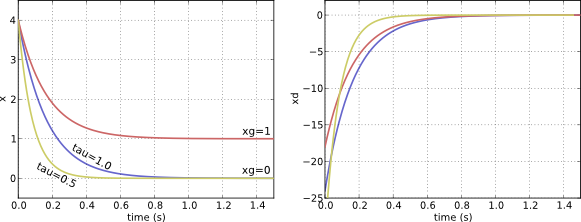
\includegraphics[height=4cm]{change_tau_attr-svg}
\caption{Changing the attractor state or time constant.}
\end{DoxyImage}
\hypertarget{page_dyn_sys_sec_dyn_sys_perturbations}{}\subsubsection{Robustness to Perturbations}\label{page_dyn_sys_sec_dyn_sys_perturbations}
Another nice feature of dynamical systems is their robustness to perturbations, which means that they will converge towards the attractor even if they are perturbed. The figure below shows how the perturbed system (cyan) converges towards the attractor state just as the unperturbed system (blue) does.


\begin{DoxyImage}
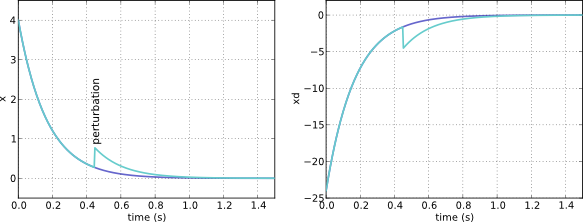
\includegraphics[height=4cm]{perturb-svg}
\caption{Perturbing the dynamical system.}
\end{DoxyImage}
\hypertarget{page_dyn_sys_sec_dyn_sys_time_constant}{}\subsubsection{Changing the speed of convergence\+: The time constant}\label{page_dyn_sys_sec_dyn_sys_time_constant}
The rates of change computed by the differential equation can be increased or decreased (leading to a faster or slower convergence) with a {\itshape time} {\itshape constant}, which is usually written as follows\+:

\begin{eqnarray*} \tau\dot{x} =& -\alpha(x-x^g)\\ \dot{x} =& (-\alpha(x-x^g))/\tau \end{eqnarray*}

{\itshape Remark}. For an exponential system, decreasing the time constant $\tau$ has the same effect as increasing $\alpha$. For more complex dynamical systems with several parameters, it is useful to have a separate parameter that changes only the speed of convergence, whilst leaving the other parameters the same.\hypertarget{page_dyn_sys_sec_dyn_sys_multi}{}\subsubsection{Multi-\/dimensional states}\label{page_dyn_sys_sec_dyn_sys_multi}
The state $x$ need not be a scalar, but may be a vector. This then represents a multi-\/dimensional state, i.\+e. $\tau\dot{\mathbf{x}} = -\alpha(\mathbf{x}-\mathbf{x}^g)$. In the code, the size of the state vector $dim(\mathbf{x})\equiv dim(\dot{\mathbf{x}})$ of a dynamical system is returned by the function Dynamical\+System\+::dim()\hypertarget{page_dyn_sys_sec_dyn_sys_autonomy}{}\subsubsection{Autonomy}\label{page_dyn_sys_sec_dyn_sys_autonomy}
Dynamical system that do not depend on time are called {\itshape autonomous}. For instance, the formula $ \dot{x} = -\alpha x$ does not depend on time, which means the exponential system is autonomous.\hypertarget{page_dyn_sys_Implementation}{}\subsubsection{Implementation}\label{page_dyn_sys_Implementation}
{\itshape  The attractor state and time constant of a dynamical system are usually passed to the constructor. They can be changed afterwards with with Dynamical\+System\+::set\+\_\+attractor\+\_\+state and Dynamical\+System\+::set\+\_\+tau. Before integration starts, the initial state can be set with Dynamical\+System\+::set\+\_\+initial\+\_\+state. This influences the output of Dynamical\+System\+::integrate\+Start, but not Dynamical\+System\+::integrate\+Step.}

{\itshape Further (first order) linear dynamical systems that are implemented in this module is a Sigmoid\+System (see \href{http://en.wikipedia.org/wiki/Exponential_decay}{\tt http\+://en.\+wikipedia.\+org/wiki/\+Exponential\+\_\+decay} and \href{http://en.wikipedia.org/wiki/Sigmoid_function}{\tt http\+://en.\+wikipedia.\+org/wiki/\+Sigmoid\+\_\+function}), as well as a dynamical system that has a constant velocity (Time\+System), so as to mimic the passing of time (time moves at a constant rate per time ;-\/)}

{\itshape  \begin{eqnarray*} \dot{x} =& -\alpha (x-x^g) & \mbox{exponential decay/growth} \label{equ_}\\ \dot{x} =& \alpha x (\beta-x) & \mbox{sigmoid} \label{equ_}\\ \dot{x} =& 1/\tau & \mbox{constant velocity (mimics the passage of time)} \label{equ_}\\ \end{eqnarray*}}

{\itshape 
\begin{DoxyImage}
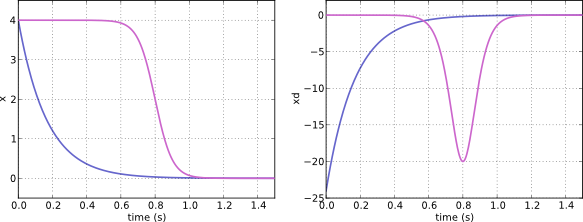
\includegraphics[height=4cm]{sigmoid-svg}
\caption{Exponential (blue) and sigmoid (purple) dynamical systems.}
\end{DoxyImage}
}

{\itshape }\hypertarget{page_dyn_sys_dyn_sys_second_order_systems}{}\subsection{Second-\/\+Order Systems}\label{page_dyn_sys_dyn_sys_second_order_systems}
The {\bfseries order} of a dynamical system is the order of the highest derivative in the differential equation. For instance, $\dot{x} = -\alpha x$ is of order 1, because the derivative with the highest order ( $\dot{x}$) has order 1. Such a system is known as a first-\/order system. All systems considered so far have been first-\/order systems, because the derivative with the highest order, i.\+e. $ \dot{x} $, has always been of order 1.\hypertarget{page_dyn_sys_dyn_sys_spring_damper}{}\subsubsection{Spring-\/\+Damper Systems}\label{page_dyn_sys_dyn_sys_spring_damper}
An example of a second order system (which also has terms $ \ddot{x} $) is a spring-\/damper system (see \href{http://en.wikipedia.org/wiki/Damped_spring-mass_system}{\tt http\+://en.\+wikipedia.\+org/wiki/\+Damped\+\_\+spring-\/mass\+\_\+system}), where $k$ is the spring constant, $c$ is the damping coefficient, and $m$ is the mass\+:

\begin{eqnarray*} m\ddot{x}=& -kx -c\dot{x} & \mbox{spring-damper (2nd order system)} \label{equ_}\\ \ddot{x}=& (-kx -c\dot{x})/m & \end{eqnarray*}\hypertarget{page_dyn_sys_dyn_sys_critical_damping}{}\subsubsection{Critical Damping}\label{page_dyn_sys_dyn_sys_critical_damping}
A spring-\/damper system is called critically damped when it converges to the attractor as quickly as possible without overshooting, as the red plot in \href{http://en.wikipedia.org/wiki/File:Damping_1.svg}{\tt http\+://en.\+wikipedia.\+org/wiki/\+File\+:\+Damping\+\_\+1.\+svg}. This happens when $c = 2\sqrt{mk}$.\hypertarget{page_dyn_sys_dyn_sys_rewrite_second_first}{}\subsubsection{Rewriting one 2nd Order Systems as two 1st Order Systems}\label{page_dyn_sys_dyn_sys_rewrite_second_first}
For implementation purposes, it is more convenient to work only with 1st order systems. Fortunately, we can expand the state $ x $ into two components $ x = [y~z]^T$ with $ z = \dot{y}$, and rewrite the differential equation as follows\+:

$ \left[ \begin{array}{l} \dot{y} \\ \dot{z} \end{array} \right] = \left[ \begin{array}{l} z \\ (-ky -cz)/m \end{array} \right] $

With this rewrite, the left term contains only first order derivatives, and the right term does not contain any derivatives. This is thus a first order system. Integrating such an expanded system is done just as one would integrate a dynamical system with a multi-\/dimensional state\+:\hypertarget{page_dyn_sys_Implementation}{}\subsubsection{Implementation}\label{page_dyn_sys_Implementation}
{\itshape  The constructor Dynamical\+System\+::\+Dynamical\+System immediately converts second order systems into first order systems with an expanded state.}

{\itshape The function Dynamical\+System\+::dim() returns the size of the entire state vector $ x = [y~z]$, the function Dynamical\+System\+::dim\+\_\+orig() return the size of only the $ y $ component. The attractor and initial state must always have the size returned by Dynamical\+System\+::dim\+\_\+orig(). } 

\chapter{Dynamical Movement Primitives}

\hypertarget{page_dmp_sec_dmp_introduction}{}\subsection{Introduction}\label{page_dmp_sec_dmp_introduction}
The core idea behind dynamical movement primitives (D\+M\+Ps) is to represent movement primitives as a combination of dynamical systems (please read \hyperlink{page_dyn_sys}{Dynamical Systems Module}, if you haven't already done so). The state variables of the main dynamical system $ [\mathbf{y \dot{y} \ddot{y}} ]$ then represent trajectories for controlling, for instance, the 7 joints of a robot arm, or its 3\+D end-\/effector position. The attractor state is the end-\/point or {\itshape goal} of the movement.

The key advantage of D\+M\+Ps is that they inherit the nice properties from linear dynamical systems (guaranteed convergence towards the attractor, robustness to perturbations, independence of time, etc) whilst allowing arbitrary (smooth) motions to be represented by adding a non-\/linear forcing term. This forcing term is often learned from demonstration, and subsequently improved through reinforcement learning.

D\+M\+Ps were introduced in {\bfseries [ijspeert02movement]}, but in this section we follow largely the notation and description in {\bfseries [ijspeert13dynamical]}, but at a slower pace.

{\itshape Historical} {\itshape remark}. Recently, the term \char`\"{}dynamic\+A\+L movement primitives\char`\"{} is preferred over \char`\"{}dynamic movement primitives\char`\"{}. The newer term makes the relation to dynamic\+A\+L systems more clear, and avoids confusion about whether the output of \char`\"{}dynamical movement primitives\char`\"{} is in kinematic or dynamic space (it is usually in kinematic space).

{\itshape Remark}. This documentation and code focusses only on discrete movement primitives. For rythmic movement primitives, we refer to {\bfseries [ijspeert13dynamical.]}\hypertarget{page_dmp_sec_core}{}\subsection{Basic Point-\/to-\/\+Point Movements\+: A Critically Damped Spring-\/\+Damper System}\label{page_dmp_sec_core}
At the heart of the D\+M\+P lies a spring-\/damper system, as described in \hyperlink{page_dyn_sys_dyn_sys_spring_damper}{Spring-\/\+Damper Systems}. In D\+M\+P papers, the notation of the spring-\/damper system is usually a bit different\+: \begin{eqnarray*} m\ddot{y} =& -ky -c\dot{y} & \mbox{spring-damper system, ``traditional notation''} \\ m\ddot{y} =& c(-\frac{k}{c}y - \dot{y})\\ \tau\ddot{y} =& \alpha(-\beta y - \dot{y}) & \mbox{with } \alpha=c,~~\beta = \frac{k}{c},~~m=\tau\\ \tau\ddot{y} =& \alpha(-\beta (y-y^g) - \dot{y})& \mbox{with attractor } y^g\\ \tau\ddot{y} =& \alpha(\beta (y^g-y) - \dot{y})& \mbox{typical DMP notation for spring-damper system}\\ \end{eqnarray*}

In the last two steps, we change the attractor state from 0 to $y^g$, where $y^g$ is the goal of the movement.

To avoid overshooting or slow convergence towards $y^g$, we prefer to have a {\itshape critically} {\itshape damped} spring-\/damper system for the D\+M\+P. For such systems $c = 2\sqrt{mk}$ must hold, see \hyperlink{page_dyn_sys_dyn_sys_critical_damping}{Critical Damping}. In our notation this becomes $\alpha = 2\sqrt{\alpha\beta}$, which leads to $\beta = \alpha/4$. This determines the value of $\beta$ for a given value of $\alpha$ in D\+M\+Ps. The influence of $\alpha$ is illustrated in the first figure in \hyperlink{page_dyn_sys_sec_dyn_sys_intro}{Introduction}.

Rewriting the second order dynamical system as a first order system (see \hyperlink{page_dyn_sys_dyn_sys_rewrite_second_first}{Rewriting one 2nd Order Systems as two 1st Order Systems}) with expanded state $ [z~y]$ yields\+:

\begin{eqnarray*} \left[ \begin{array}{l} {\dot{z}} \\ {\dot{y}} \end{array} \right] = \left[ \begin{array}{l} (\alpha (\beta({y}^{g}-{y})-{z}))/\tau \\ {z}/\tau \end{array} \right] \mbox{~~~~with init. state~} \left[ \begin{array}{l} 0 \\ y_0 \end{array} \right] \mbox{~and attr. state~} \left[ \begin{array}{l} {0} \\ {y}^g \end{array} \right] \end{eqnarray*}

Please note that in the implementation, the state is implemented as $ [y~z]$. The order is inconsequential, but we use the notation above ( $[z~y]$) throughout the rest of this tutorial section, for consistency with the D\+M\+P literature.\hypertarget{page_dmp_sec_forcing}{}\subsection{Arbitrary Smooth Movements\+: the Forcing Term}\label{page_dmp_sec_forcing}
The representation described in the previous section has some nice properties in terms of \hyperlink{page_dyn_sys_sec_dyn_sys_convergence}{Convergence towards the Attractor} , \hyperlink{page_dyn_sys_sec_dyn_sys_perturbations}{Robustness to Perturbations} , and \hyperlink{page_dyn_sys_sec_dyn_sys_autonomy}{Autonomy}, but it can only represent very simple movements. To achieve more complex movements, we add a time-\/dependent forcing term to the spring-\/damper system. The spring-\/damper systems and forcing term are together known as a {\itshape transformation} {\itshape system}.

\begin{eqnarray*} \left[ \begin{array}{l} {\dot{z}} \\ {\dot{y}} \end{array} \right] = \left[ \begin{array}{l} (\alpha (\beta({y}^{g}-{y})-{z}) + f(t))/\tau \\ {z}/\tau \end{array} \right] \mbox{~~~~with init. state~} \left[ \begin{array}{l} 0 \\ y_0 \end{array} \right] \mbox{~and attr. state~} \left[ \begin{array}{l} {?} \\ {y}^g \end{array} \right] \end{eqnarray*}

The forcing term is an open loop controller, i.\+e. it depends only on time. By modifying the acceleration profile of the movement with a forcing term, arbitrary smooth movements can be achieved. The function $ f(t)$ is usually a function approximator, such as locally weighted regression (L\+W\+R) or locally weighted projection regression (L\+W\+P\+R), see \hyperlink{page_func_approx}{Function Approximation Module}. The graph below shows an example of a forcing term implemented with L\+W\+R with random weights for the basis functions.


\begin{DoxyImage}
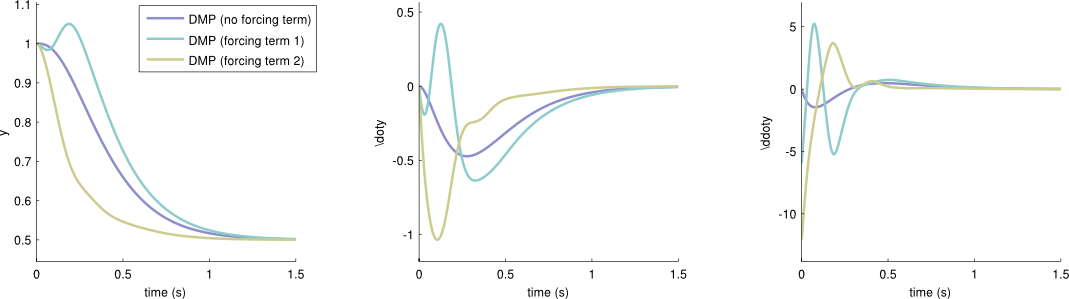
\includegraphics[height=4cm]{dmp_forcing_terms-svg}
\caption{A non-\/linear forcing term enable more complex trajectories to be generated (these D\+M\+Ps use a goal system and an exponential gating term).}
\end{DoxyImage}
\hypertarget{page_dmp_sec_forcing_convergence}{}\subsubsection{Ensuring Convergence to 0 of the Forcing Term\+: the Gating System}\label{page_dmp_sec_forcing_convergence}
Since we add a forcing term to the dynamical system, we can no longer guarantee that the system will converge towards $ x^g $; perhaps the forcing term continually pushes it away $ x^g $ (perhaps it doesn't, but the point is that we cannot {\itshape guarantee} that it {\itshape always} doesn't). That is why there is a question mark in the attractor state in the equation above. To guarantee that the movement will always converge towards the attractor $ x^g $, we need to ensure that the forcing term decreases to 0 towards the end of the movement. To do so, a gating term is added, which is 1 at the beginning of the movement, and 0 at the end. This gating term itself is determined by, of course, a dynamical system. In {\bfseries [ijspeert02movement]}, it was suggested to use an exponential system. We add this extra system to our dynamical system by expanding the state as follows\+:

\begin{eqnarray*} \dot{x} = \left[ \begin{array}{l} {\dot{z}} \\ {\dot{y}} \\ {\dot{x}} \end{array} \right] = \left[ \begin{array}{l} (\alpha_y (\beta_y({y}^{g}-{y})-{z}) + x\cdot f(t))/\tau \\ {z}/\tau \\ -\alpha_x x/\tau \end{array} \right] \mbox{~~~~with init. state~} \left[ \begin{array}{l} 0 \\ y_0 \\ 1 \end{array} \right] \mbox{~and attr. state~} \left[ \begin{array}{l} {0} \\ {y}^g \\ 0 \end{array} \right] \end{eqnarray*}\hypertarget{page_dmp_sec_forcing_autonomy}{}\subsubsection{Ensuring Autonomy of the Forcing Term\+: the Phase System}\label{page_dmp_sec_forcing_autonomy}
By introducing the dependence of the forcing term $ f(t)$ on time $ t $ the overall system is no longer autonomous. To achieve independence of time, we therefore let $ f $ be a function of the state of an (autonomous) dynamical system rather than of $ t $. This system represents the {\itshape phase} of the movement. {\bfseries [ijspeert02movement]} suggested to use the same dynamical system for the gating and phase, and use the term {\itshape canonical} {\itshape system} to refer this joint gating/phase system. Thus the phase of the movement starts at 1, and converges to 0 towards the end of the movement, just like the gating system. The new formulation now is (the only difference is $ f(x)$ instead of $ f(t)$)\+:

\begin{eqnarray*} \left[ \begin{array}{l} {\dot{z}} \\ {\dot{y}} \\ {\dot{x}} \end{array} \right] = \left[ \begin{array}{l} (\alpha_y (\beta_y({y}^{g}-{y})-{z}) + x\cdot f(x))/\tau \\ {z}/\tau \\ -\alpha_x x/\tau \end{array} \right] \mbox{~~~~with init. state~} \left[ \begin{array}{l} 0 \\ y_0 \\ 1 \end{array} \right] \mbox{~and attr. state~} \left[ \begin{array}{l} {0} \\ {y}^g \\ 0 \end{array} \right] \end{eqnarray*}

\begin{DoxyRefDesc}{Todo}
\item[\hyperlink{todo__todo000006}{Todo}]Discuss goal-\/dependent scaling, i.\+e. $ f(t)s(x^g-x_0) $?\end{DoxyRefDesc}
\hypertarget{page_dmp_sec_multidim_dmp}{}\subsubsection{Multi-\/dimensional Dynamic Movement Primitives}\label{page_dmp_sec_multidim_dmp}
Since D\+M\+Ps usually have multi-\/dimensional states (e.\+g. one output $ {\mathbf{y}}_{d=1\dots D}$ for each of the $ D $ joints), it is more accurate to use bold fonts for the state variables (except the gating/phase system, because it is always 1\+D) so that they represent vectors\+:

\begin{eqnarray*} \left[ \begin{array}{l} {\dot{\mathbf{z}}} \\ {\dot{\mathbf{y}}} \\ {\dot{x}} \end{array} \right] = \left[ \begin{array}{l} (\alpha_y (\beta_y({\mathbf{y}}^{g}-\mathbf{y})-\mathbf{z}) + x\cdot f(x))/\tau \\ \mathbf{z}/\tau \\ -\alpha_x x/\tau \end{array} \right] \mbox{~~~~with init. state~} \left[ \begin{array}{l} \mathbf{0} \\ \mathbf{z}_0 \\ 1 \end{array} \right] \mbox{~and attr. state~} \left[ \begin{array}{l} \mathbf{0} \\ \mathbf{y}^g \\ 0 \end{array} \right] \end{eqnarray*}

So far, the graphs have shown 1-\/dimensional systems. To generate D-\/dimensional trajectories for, for instance, the 7 joints of an arm or the 3\+D position of its end-\/effector, we simply use D transformation systems. A key principle in D\+M\+Ps is to use one and the same phase system for all of the transformation systems, to ensure that the output of the transformation systems are synchronized in time. The image below show the evolution of all the dynamical systems involved in integrating a multi-\/dimensional D\+M\+P.


\begin{DoxyImage}
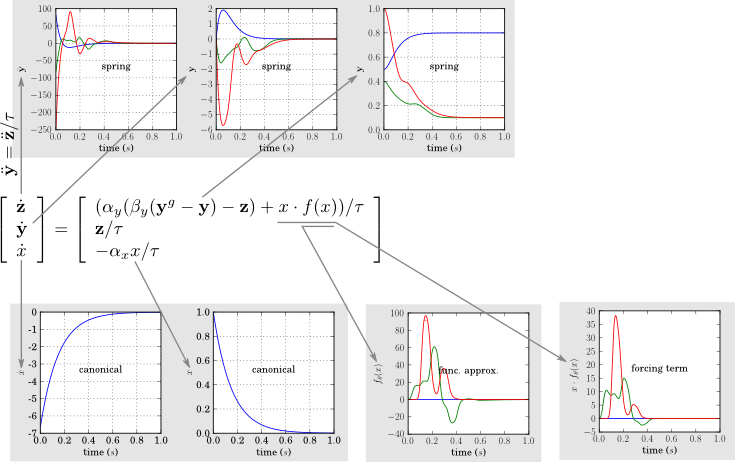
\includegraphics[height=8cm]{dmpplot_ijspeert2002movement-svg}
\caption{The various dynamical systems and forcing terms in multi-\/dimensional D\+M\+Ps.}
\end{DoxyImage}


{\itshape }

{\itshape }\hypertarget{page_dyn_sys_Implementation}{}\subsubsection{Implementation}\label{page_dyn_sys_Implementation}
{\itshape  Since a Dynamical Movement Primitive is a dynamical system, the Dmp class derives from the Dynamical\+System class. It overrides the virtual function Dynamical\+System\+::integrate\+Start(). Integrating the D\+M\+P numerically (Euler or 4th order Runge-\/\+Kutta) is done with the generic Dynamical\+System\+::integrate\+Step() function. It also implements the pure virtual function Dynamical\+System\+::analytical\+Solution(). Because a D\+M\+P cannot be solved analytically (we cannot write it in closed form due to the arbitrary forcing term), calling Dmp\+::analytical\+Solution() in fact performs a numerical Euler integration (although the linear subsystems (phase, gating, etc.) are analytically solved because this is faster computationally).}

{\itshape Please note that in this tutorial we have used the notation $[z~y]$ for consistency with the D\+M\+P literature. In the C++ implementation, the order is rather $[y~z]$.}

{\itshape {\itshape Remark}. Dmp inherits the function Dynamical\+System\+::integrate\+Step() from the Dynamical\+System class. Dynamical\+System\+::integrate\+Step() uses either Euler integration, or 4-\/th order Runge-\/\+Kutta. The latter is more accurate, but requires 4 calls of Dynamical\+System\+::differential\+Equation() instead of 1). Which one is used can be set with Dynamical\+System\+::set\+\_\+integration\+\_\+method(). To numerically integrate a dynamical system, one must carefully choose the integration time dt. Choosing it too low leads to inaccurate integration, and the numerical integration will diverge from the 'true' solution acquired through analytical solution. See \href{http://en.wikipedia.org/wiki/Euler%27s_method}{\tt http\+://en.\+wikipedia.\+org/wiki/\+Euler\%27s\+\_\+method} for examples. Choosing dt depends entirely on the time-\/scale (seconds vs. years) and parameters of the dynamical system (time constant, decay parameters). For D\+M\+Ps, which are expected to take between 0.\+5-\/10 seconds, dt is usually chosen to be in the range 0.\+01-\/0.\+001. }\hypertarget{page_dmp_sec_dmp_alternative}{}\subsection{Alternative Systems for Gating, Phase and Goals}\label{page_dmp_sec_dmp_alternative}
\hypertarget{page_dmp_sec_dmp_sigmoid_gating}{}\subsubsection{Gating\+: Sigmoid System}\label{page_dmp_sec_dmp_sigmoid_gating}
A disadvantage of using an exponential system as a gating term is that the gating decreases very quickly in the beginning. Thus, the output of the function approximator $ f(x) $ needs to be very high towards the end of the movement if it is to have any effect at all. This leads to scaling issues when training the function approximator.

Therefore, sigmoid systems have more recently been proposed {\bfseries [kulvicius12joining]} as a gating system. This leads to the following D\+M\+P formulation (since the gating and phase system are no longer shared, we introduce a new state variable $ v $ for the gating term\+:

\begin{eqnarray*} \left[ \begin{array}{l} {\dot{\mathbf{z}}} \\ {\dot{\mathbf{y}}} \\ {\dot{x}} \\ {\dot{v}} \end{array} \right] = \left[ \begin{array}{l} (\alpha_y (\beta_y({\mathbf{y}}^{g}-\mathbf{y})-\mathbf{z}) + v\cdot f(x))/\tau \\ \mathbf{z}/\tau \\ -\alpha_x x/\tau \\ -\alpha_v v (1-v/v_{\mbox{\scriptsize max}}) \end{array} \right] \mbox{~~~~with init. state~} \left[ \begin{array}{l} \mathbf{0} \\ \mathbf{y}_0 \\ 1 \\ 1 \end{array} \right] \mbox{~and attr. state~} \left[ \begin{array}{l} \mathbf{0} \\ \mathbf{y}^g \\ 0 \\ 0 \end{array} \right] \end{eqnarray*}

where the term $ v_{\mbox{\scriptsize max}}$ is determined by $\tau $\hypertarget{page_dmp_sec_dmp_phase}{}\subsubsection{Phase\+: Constant Velocity System}\label{page_dmp_sec_dmp_phase}
In practice, using an exponential phase system may complicate imitation learning of the function approximator $ f $, because samples are not equidistantly spaced in time. Therefore, we introduce a dynamical system that mimics the properties of the phase system described in {\bfseries [kulvicius12joining]}, whilst allowing for a more natural integration in the D\+M\+P formulation, and thus our code base. This system starts at 0, and has a constant velocity of $1/\tau$, which means the system reaches 1 when $t=\tau$. When this point is reached, the velocity is set to 0.

\begin{eqnarray*} \dot{x} =& 1/\tau \mbox{~if~} x < 1 & \\ & 0 \mbox{~if~} x>1 \\ \end{eqnarray*}

This, in all honesty, is a bit of a hack, because it leads to a non-\/smooth acceleration profile. However, its properties as an input to the function approximator are so advantageous that we have designed it in this way (the implementation of this system is in the Time\+System class).


\begin{DoxyImage}
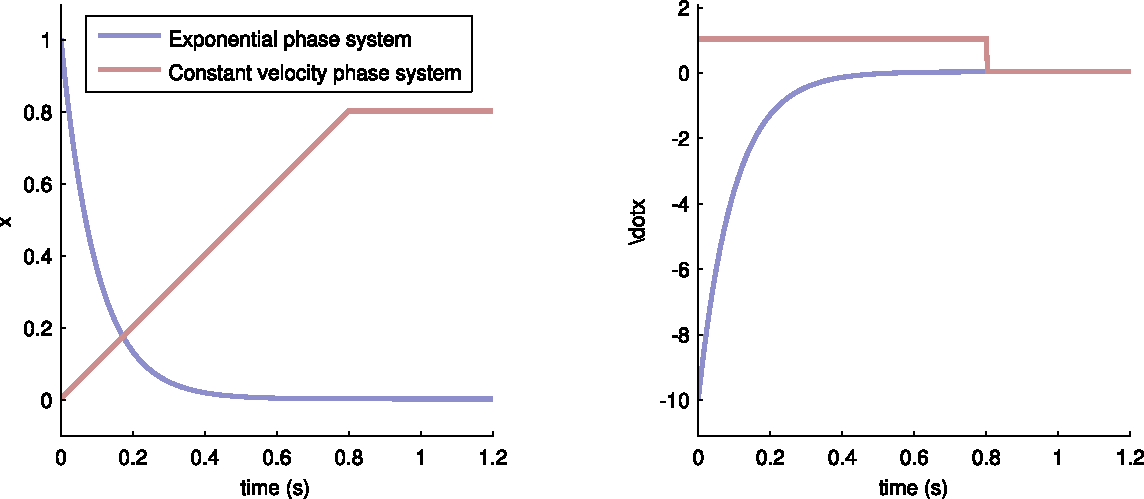
\includegraphics[height=4cm]{phase_systems-svg}
\caption{Exponential and constant velocity dynamical systems as the 1\+D phase for a dynamical movement primitive.}
\end{DoxyImage}


With the constant velocity dynamical system the D\+M\+P formulation becomes\+:

\begin{eqnarray*} \left[ \begin{array}{l} {\dot{\mathbf{z}}} \\ {\dot{\mathbf{y}}} \\ {\dot{x}} \\ {\dot{v}} \end{array} \right] = \left[ \begin{array}{l} (\alpha_y (\beta_y({\mathbf{y}}^{g}-\mathbf{y})-\mathbf{z}) + v\cdot f(x))/\tau \\ \mathbf{z}/\tau \\ 1/\tau \\ -\alpha_v v (1-v/v_{\mbox{\scriptsize max}}) \end{array} \right] \mbox{~~~~with init. state~} \left[ \begin{array}{l} \mathbf{0} \\ \mathbf{y}_0 \\ 0 \\ 1 \end{array} \right] \mbox{~and attr. state~} \left[ \begin{array}{l} \mathbf{0} \\ \mathbf{y}^g \\ 1 \\ 0 \end{array} \right] \end{eqnarray*}\hypertarget{page_dmp_sec_delayed_goal}{}\subsubsection{Zero Initial Accelerations\+: the Delayed Goal System}\label{page_dmp_sec_delayed_goal}
Since the spring-\/damper system leads to high initial accelerations (see the graph to the right below), which is usually not desirable for robots, it was suggested to move the attractor of the system from the initial state $ y_0 $ to the goal state $ y^g $ {\itshape during} the movement {\bfseries [kulvicius12joining.]} This delayed goal attractor $ y^{g_d} $ itself is represented as an exponential dynamical system that starts at $ y_0 $, and converges to $ y^g $ (in early versions of D\+M\+Ps, there was no delayed goal system, and $ y^{g_d} $ was simply equal to $ y^g $ throughout the movement). The combination of these two systems, listed below, leads to a movement that starts and ends with 0 velocities and accelerations, and approximately has a bell-\/shaped velocity profile. This representation is thus well suited to generating human-\/like point-\/to-\/point movements, which have similar properties.

\begin{eqnarray*} \left[ \begin{array}{l} {\dot{\mathbf{z}}} \\ {\dot{\mathbf{y}}} \\ {\dot{\mathbf{y}}^{g_d}} \\ {\dot{x}} \\ {\dot{v}} \end{array} \right] = \left[ \begin{array}{l} (\alpha_y (\beta_y({\mathbf{y}}^{g_d}-\mathbf{y})-\mathbf{z}) + v\cdot f(x))/\tau \\ \mathbf{z}/\tau \\ -\alpha_g({\mathbf{y}^g-\mathbf{y}^{g_d}}) \\ 1/\tau \\ -\alpha_v v (1-v/v_{\mbox{\scriptsize max}}) \end{array} \right] \mbox{~~~~with init. state~} \left[ \begin{array}{l} \mathbf{0} \\ \mathbf{y}_0 \\ \mathbf{y}_0 \\ 0 \\ 1 \end{array} \right] \mbox{~and attr. state~} \left[ \begin{array}{l} \mathbf{0} \\ \mathbf{y}^g \\ \mathbf{y}^g \\ 1 \\ 0 \end{array} \right] \end{eqnarray*}


\begin{DoxyImage}
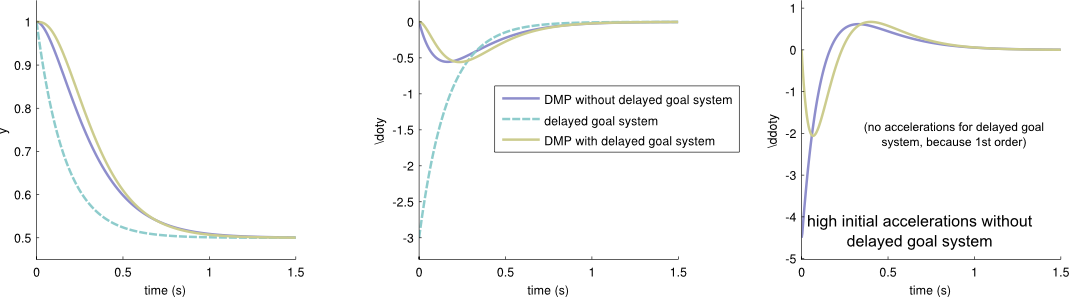
\includegraphics[height=4cm]{dmp_and_goal_system-svg}
\caption{A first dynamical movement primitive, with and without a delayed goal system (left\+: state variable, center\+: velocities, right\+: accelerations.}
\end{DoxyImage}


In my experience, this D\+M\+P formulation is the best for learning human-\/like point-\/to-\/point movements (bell-\/shaped velocity profile, approximately zero velocities and accelerations at beginning and start of the movement), and generates nice normalized data for the function approximator without scaling issues (an exact empirical evaluation is on the stack...). The image below shows the interactions between the spring-\/damper system, delayed goal system, phase system and gating system.


\begin{DoxyImage}
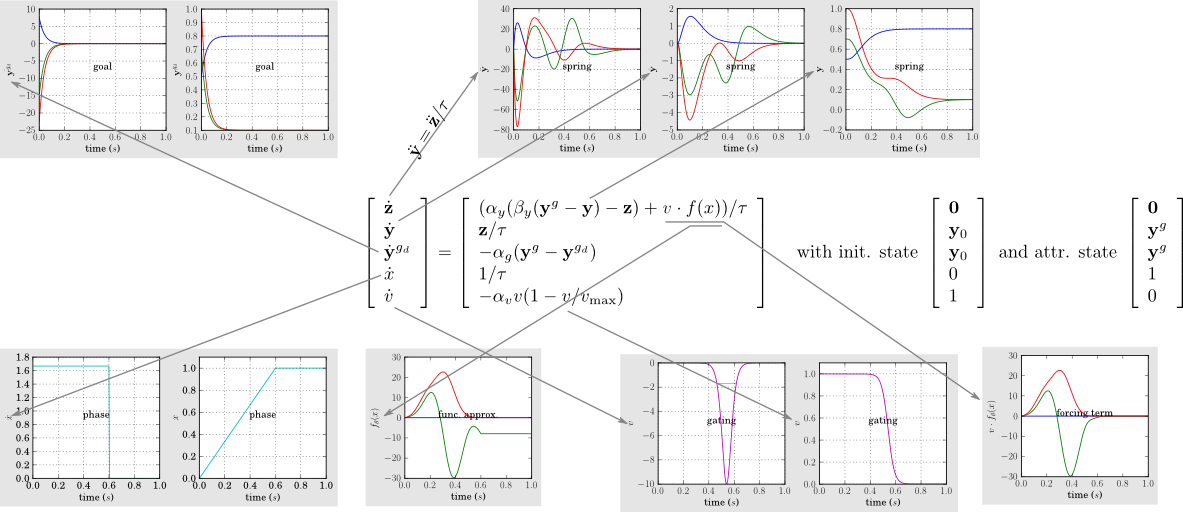
\includegraphics[height=7cm]{dmpplot_kulvicius2012joining-svg}
\caption{The various dynamical systems and forcing terms in multi-\/dimensional D\+M\+Ps.}
\end{DoxyImage}
\hypertarget{page_dmp_sec_dmp_issues}{}\subsection{Known Issues}\label{page_dmp_sec_dmp_issues}
\begin{DoxyRefDesc}{Todo}
\item[\hyperlink{todo__todo000007}{Todo}]Known Issues\end{DoxyRefDesc}


\begin{DoxyItemize}
\item Scaling towards novel goals\end{DoxyItemize}
\hypertarget{page_dmp_sec_dmp_summary}{}\subsection{Summary}\label{page_dmp_sec_dmp_summary}
The core idea in dynamical movement primitives is to combine dynamical systems, which have nice properties in terms of convergence towards the goal, robustness to perturbations, and independence of time, with function approximators, which allow for the generation of arbitrary (smooth) trajectories. The key enabler to this approach is to gate the output of the function approximator with a gating system, which is 1 at the beginning of the movement, and 0 towards the end.

Further enhancements can be made by making the system autonomous (by using the output of a phase system rather than time as an input to the function approximator), or having initial velocities and accelerations of 0 (by using a delayed goal system).

Multi-\/dimensional D\+M\+Ps are achieved by using multi-\/dimensional dynamical systems, and learning one function approximator for each dimension. Synchronization of the different dimensions is ensure by coupling them with only {\itshape one} phase system. 

\bibliographystyle{apalike}
\bibliography{../dmp}


\chapter{Function Approximation for the Forcing Term}

(Please note that the the tutorial on Dynamical Movement Primitives is now basically over. The rest is more about documentation of the code.)

\hypertarget{page_func_approx_sec_fa}{}\subsection{Function Approximation}\label{page_func_approx_sec_fa}
This module implements a set of function approximators, i.\+e. supervised learning algorithms that are trained with demonstration pairs input/target, after which they make predictions for new inputs. For simplicity, this module implements only batch learning (not incremental), and does not allow trained function approximators to be retrained.

The two main functions are Function\+Approximator\+::train, which takes a set of inputs and corresponding targets, and Function\+Approximator\+::predict, which makes predictions for novel inputs.\hypertarget{page_func_approx_sec_fa_metaparameters}{}\subsubsection{Meta\+Parameters and Model\+Parameters}\label{page_func_approx_sec_fa_metaparameters}
In this module, algorithmic parameters are called Meta\+Parameters, and the parameters of the model when the function approximator has been trained are called Model\+Parameters. The rationale for this is that an untrained function approximator can be entirely reconstructed if its Meta\+Parameters are known; this is useful for saving to file and making copies. A trained function approximator can be compeletely reconstructed given only its Model\+Parameters.

The life-\/cycle of a function approximator is as follows\+:

{\bfseries 1}. {\bfseries Initialization\+:} The function approximator is initialized by calling the constructor with the Meta\+Parameters. Its Model\+Parameters are set to N\+U\+L\+L, indicating that the model is untrained.

{\bfseries 2}. {\bfseries Training\+:} Function\+Approximator\+::train is called, which performs the conversion\+: $ \mbox{train}: \mbox{MetaParameters} \times \mbox{Inputs} \times \mbox{Targets} \mapsto \mbox{ModelParameters} $

{\bfseries 3}. {\bfseries Prediction\+:} Function\+Approximator\+::predict is called, which performs the conversion\+: $ \mbox{predict}: \mbox{ModelParameters} \times \mbox{Input} \mapsto \mbox{Output}$

{\itshape Remark}. Function\+Approximator\+::train in Step {\bfseries 2}. may only be called once. If you explicitly want to retrain the function approximator with novel input/target data call Function\+Approximator\+::re\+Train() instead.

{\itshape Remark}. During the initialization, Model\+Parameters may also be passed to the constructor. This means that an already trained function approximator is initialized. Step {\bfseries 2}. above is thus skipped.\hypertarget{page_func_approx_sec_fa_changing_modelparameters}{}\subsubsection{Changing the Model\+Parameters of a Function\+Approximator}\label{page_func_approx_sec_fa_changing_modelparameters}
The user should not be allowed to set the Model\+Parameters of a trained function approximator directly. Hence, Function\+Approximator\+::set\+Model\+Parameters is protected. However, in order to change the values inside the model parameters (for instance when optimizing them), the user may call Model\+Parameters\+::get\+Parameter\+Vector\+Selected and Model\+Parameters\+::set\+Parameter\+Vector\+Selected it inherits these functions from Parameterizable). These take a vector of doubles, check if the vector has the right size, and get/set the Model\+Parameters accordingly.

Function approximators often have different types of model parameters. For instance, the model parameters of Locally Weighted Regression (Function\+Approximator\+L\+W\+R) represent the centers and widths of the basis functions, as well as the slopes of the line segments. If you only want to get/set the slopes when calling Model\+Parameters\+::get\+Parameter\+Vector\+Selected and Model\+Parameters\+::set\+Parameter\+Vector\+Selected, you must use Model\+Parameters\+::set\+Selected\+Parameters(const std\+::set$<$std\+::string$>$\& selected\+\_\+values\+\_\+labels), for instance as follows\+:


\begin{DoxyCode}
std::set<std::string> selected;
selected.insert(\textcolor{stringliteral}{"slopes"});
model\_parameters.setSelectedParameters(selected);
Eigen::VectorXd values;
model\_parameters.getParameterVectorSelected(values);
\textcolor{comment}{// "values" now only contains the slopes of the line segments}

selected.clear();
selected.insert(\textcolor{stringliteral}{"centers"});
selected.insert(\textcolor{stringliteral}{"slopes"});
model\_parameters.setSelectedParameters(selected);
model\_parameters.getParameterVectorSelected(values);
\textcolor{comment}{// "values" now contains the centers of the basis functions AND slopes of the line segments}
\end{DoxyCode}


The rationale behind this implementation is that optimizers (such as evolution strategies) should not have to care about whether a particular set of model parameters contains centers, widths or slopes. Therefore, these different types of parameters are provided in one vector without semantics, and the generic interface is provided by the Parameterizable class.

Classes that inherit from Parameterizable (such as all Model\+Parameters and Function\+Approximator subclasses, must implement the pure virtual methods Parameterizable\+::get\+Parameter\+Vector\+All Parameterizable\+::set\+Parameter\+Vector\+All and Parameterizable\+::get\+Parameter\+Vector\+Mask. Which gets/sets all the possible parameters in one vector, and a mask specifying the semantics of each value in the vector. The work of setting/getting the selected parameters (and normalizing them) is done in the Parameterizable class itself. This approach is a slightly longer run-\/time than doing the work in the subclasses, but it leads to more legible and robust code (less code duplication).\hypertarget{page_func_approx_sec_caching_basisfunctions}{}\subsubsection{Caching of basis functions}\label{page_func_approx_sec_caching_basisfunctions}
If the parameters of the basis functions (centers and widths of the kernels) do not change often, you can cache the basis function activations by calling Model\+Parameters\+::set\+\_\+caching(true). This can lead to speed improvements because the activations are not computed over and over again. This function only makes senses if the inputs remain the same, i.\+e. this is not the case when running on a real robot.

The reason why caching is implemented in Model\+Parameters, and not in Function\+Approximator is because Model\+Parameters knows which parts of the Model\+Parameters change the basis function activations, and which do not (for instance in R\+B\+F\+N, the widths and centers change the basis function activations, but the weights do not). 

\chapter{Black-box Optimization with Evolution Strategies}

This module implements several \href{http://en.wikipedia.org/wiki/Evolution_strategy}{\tt evolution strategies} for the \href{http://en.wikipedia.org/wiki/Optimization_%28mathematics%29}{\tt optimization} of black-\/box \href{http://en.wikipedia.org/wiki/Loss_function}{\tt cost functions}.

Black-\/box in this context means that no assumptions about the cost function can be made, for example, we do not have access to its derivative, and we do not even know if it is continuous or not.

The evolution strategies that are implemented are all based on reward-\/weighted averaging (aka probablity-\/weighted averaging), as explained in this paper/presentation\+: \href{http://icml.cc/discuss/2012/171.html}{\tt http\+://icml.\+cc/discuss/2012/171.\+html}

The basic algorithm is as follows\+: 
\begin{DoxyCode}
x\_mu = ??; x\_Sigma = ?? \textcolor{comment}{// Initialize multi-variate Gaussian distribution}
\textcolor{keywordflow}{while} (!halt\_condition) \{

    \textcolor{comment}{// Explore}
    \textcolor{keywordflow}{for} k=1:K \{
        x[k]     ~ N(x\_mu,x\_Sigma)    \textcolor{comment}{// Sample from Gaussian}
        costs[k] = costfunction(x[k]) \textcolor{comment}{// Evaluate sample}
    \}
        
    \textcolor{comment}{// Update distribution}
    weights = costs2weights(costs) \textcolor{comment}{// Should assign higher weights to lower costs}
    x\_mu\_new = weights^T * x; \textcolor{comment}{// Compute weighted mean of samples}
    x\_covar\_new = (weights .* x)^T * weights \textcolor{comment}{// Compute weighted covariance matrix of samples}
    
    x\_mu = x\_mu\_new
    x\_covar = x\_covar\_new
\}
\end{DoxyCode}
\hypertarget{page_bbo_sec_bbo_implementation}{}\subsection{Implementation}\label{page_bbo_sec_bbo_implementation}
The algorithm above has been implemented as follows (see run\+Evolutionary\+Optimization() and \hyperlink{demoEvolutionaryOptimization_8cpp}{demo\+Evolutionary\+Optimization.\+cpp})\+: 
\begin{DoxyCode}
\textcolor{keywordtype}{int} n\_dim = 2; \textcolor{comment}{// Optimize 2D problem}

\textcolor{comment}{// This is the cost function to be optimized}
CostFunction* cost\_function = \textcolor{keyword}{new} CostFunctionQuadratic(VectorXd::Zero(n\_dim));

\textcolor{comment}{// This is the initial distribution}
DistributionGaussian* distribution = \textcolor{keyword}{new} DistributionGaussian(VectorXd::Random(n\_dim),MatrixXd::Identity(
      n\_dim)) 

\textcolor{comment}{// This is the updater which will update the distribution}
double eliteness = 10.0;
Updater* updater = new UpdaterMean(eliteness);

\textcolor{comment}{// Some variables}
MatrixXd samples;
VectorXd costs;

for (\textcolor{keywordtype}{int} i\_update=1; i\_update<=n\_updates; i\_update++)
\{
  
    \textcolor{comment}{// 1. Sample from distribution}
    \textcolor{keywordtype}{int} n\_samples\_per\_update = 10;
    distribution->generateSamples(n\_samples\_per\_update, samples);
  
    \textcolor{comment}{// 2. Evaluate the samples}
    cost\_function->evaluate(samples,costs);
  
    \textcolor{comment}{// 3. Update parameters}
    updater->updateDistribution(*distribution, samples, costs, *distribution);
    
\}
\end{DoxyCode}
\hypertarget{page_bbo_sec_bbo_task_and_task_solver}{}\subsubsection{Cost\+Function vs Task/\+Task\+Solver}\label{page_bbo_sec_bbo_task_and_task_solver}
When the cost function has a simple structure, e.\+g. cost = $ x^2 $ it is convenient to implement the function $ x^2 $ in Cost\+Function\+::evaluate(). In robotics however, it is more suitable to make the distinction between a task (e.\+g. lift an object), and an entity that solves this task (e.\+g. your robot, my robot, a simulated robot, etc.). For these cases, the Cost\+Function is split into a Task and a Task\+Solver, as follows\+:


\begin{DoxyCode}
CostFunction::evaluate(samples,costs) \{
  TaskSolver::performRollouts(samples,cost\_vars)
  Task::evaluate(cost\_vars,costs)
\}
\end{DoxyCode}


The idea here is that the Task\+Solver uses the samples to perform a rollout (e.\+g. the samples represent the parameters of a policy which is executed) and computes all the variables that are relevant to determining the cost (e.\+g. it records the forces at the robot's end-\/effector, if this is something that needs to be minimized)

Some further advantages of this approach\+: \begin{DoxyItemize}
\item Different robots can solve the exact same Task implementation of the same task. \item Robots do not need to know about the cost function to perform rollouts (and they shouldn't) \item The intermediate cost-\/relevant variables can be stored to file for visualization etc. \item The procedures for performing the roll-\/outs (on-\/line on a robot) and doing the evaluation/updating/sampling (off-\/line on a computer) can be seperated, because there is a separate Task\+Solver\+::perform\+Rollouts function.\end{DoxyItemize}
When using the Task/\+Task\+Solver approach, the run\+Evolutionary\+Optimization process is as follows (only minor changes to the above)\+: 
\begin{DoxyCode}
\textcolor{keywordtype}{int} n\_dim = 2; \textcolor{comment}{// Optimize 2D problem}

\textcolor{comment}{// This is the cost function to be optimized}
CostFunction* cost\_function = \textcolor{keyword}{new} CostFunctionQuadratic(VectorXd::Zero(n\_dim));

\textcolor{comment}{// This is the initial distribution}
DistributionGaussian* distribution = \textcolor{keyword}{new} DistributionGaussian(VectorXd::Random(n\_dim),MatrixXd::Identity(
      n\_dim)) 

\textcolor{comment}{// This is the updater which will update the distribution}
double eliteness = 10.0;
Updater* updater = new UpdaterMean(eliteness);

\textcolor{comment}{// Some variables}
MatrixXd samples;
VectorXd costs;

for (\textcolor{keywordtype}{int} i\_update=1; i\_update<=n\_updates; i\_update++)
\{
  
    \textcolor{comment}{// 1. Sample from distribution}
    \textcolor{keywordtype}{int} n\_samples\_per\_update = 10;
    distribution->generateSamples(n\_samples\_per\_update, samples);
  
    \textcolor{comment}{// 2A. Perform the roll-outs}
    task\_solver->performRollouts(samples,cost\_vars);
  
    \textcolor{comment}{// 2B. Evaluate the samples}
    task->evaluate(cost\_vars,costs);
  
    \textcolor{comment}{// 3. Update parameters}
    updater->updateDistribution(*distribution, samples, costs, *distribution);
    
\}
\end{DoxyCode}
 

%\chapter{Black-box Optimization of Dynamical Movement Primitives}
%
%\input{ ../../build_dir/docs/latex/page_dmp_bbo}



\end{document}
